% Copyright 2010 by Nicholas Bartlett

\documentclass{beamer}
\usepackage{algorithm}
\usepackage{algorithmic}
\usepackage[numbers]{natbib}

% Setup appearance:

\usetheme{Darmstadt}
%\usetheme{Copenhagen}
\usefonttheme[onlylarge]{structurebold}
\setbeamerfont*{frametitle}{size=\normalsize,series=\bfseries}
\setbeamertemplate{navigation symbols}{}

% Standard packages
\usepackage[english]{babel}
%\usepackage[latin1]{inputenc}
%\usepackage{times}
%\usepackage[T1]{fontenc}
%\usepackage{nnfootnote}
\usepackage{amsfonts}
\usepackage{amsmath}
%\newcommand{\argmax}{\operatornamewithlimits{argmax}}
\def\newblock{\hskip .11em plus .33em minus .07em}
% Setup TikZ

%\usepackage{tikz}
%\usetikzlibrary{arrows}
%\tikzstyle{block}=[draw opacity=0.7,line width=1.4cm]

\bibliographystyle{plainnat}

% Author, Title, etc.

\title[Forgetting Counts: A Constant Memory Approach to Online Prediction of a Discrete Sequence] 
{
	Forgetting Counts
}

\author[Bartlett]
{
  Nicholas~Bartlett \\ {\tiny joint work with David~Pfau and Frank~Wood } %\inst{1}
}

\institute[Columbia University]
{
  %\inst{1}%
  Columbia University
}

%\date[Apr 17, 2010]
%{Apr 17, 2010}

%\def\blfootnote{\xdef\@thefnmark{}\@footnotetext}

% The main document
% !TEX root = talk.tex

\newcommand{\comment}[1]{}
%\newcommand{\comment}[1]{{\marginpar{\tiny {#1} }}}
\def\todo#1{TODO(#1)}

\def\bigO{{\mathcal O}}
\def\balpha{\mbox{\boldmath $\alpha$}}
\def\bbeta{\mbox{\boldmath $\beta$}}
\def\beeta{\mbox{\boldmath $\eta$}}
\def\blambda{\mbox{\boldmath $\lambda$}}
\def\bmu{\mbox{\boldmath $\mu$}}
\def\bphi{\mbox{\boldmath $\phi$}}
\def\bpsi{\mbox{\boldmath $\psi$}}
\def\bsigma{\mbox{\boldmath $\sigma$}}
\def\btau{\mbox{\boldmath $\tau$}}
\def\btheta{\mbox{\boldmath $\theta$}}
\def\dbphi{\dot{\mbox{\boldmath $\phi$}}}
\def\dbtau{\dot{\mbox{\boldmath $\tau$}}}
\def\dbtheta{\dot{\mbox{\boldmath $\theta$}}}

%\newcommand{\nofootnotemark}{\let\@makefnmark\relax}
\newcommand{\bX}{\mathbf{X}}
\newcommand{\bY}{\mathbf{Y}}
\newcommand{\bW}{\mathbf{W}}
\newcommand{\bZ}{\mathbf{Z}}
\newcommand{\bH}{\mathbf{H}}
\newcommand{\bQ}{\mathbf{Q}}
\newcommand{\bA}{\mathbf{A}}
\newcommand{\bI}{\mathbf{I}}
\newcommand{\by}{\mathbf{y}}
\newcommand{\bz}{\mathbf{z}}
\newcommand{\bx}{\mathbf{x}}

\newcommand{\ith}{i^\mathrm{th}}
\def\A{{\bf A}}
\def\B{{\bf B}}
\def\C{{\bf C}}
\def\D{{\bf D}}
\def\F{{\bf F}}
\def\L{{\bf L}}
\def\M{{\bf M}}
\def\W{{\bf W}}
\def\I{{\bf I}}
\def\J{{\bf J}}
\def\R{{\bf R}}
\def\U{{\bf U}}
\def\V{{\bf V}}
\def\b{{\bf b}}
\def\c{{\bf c}}
\def\d{{\bf d}}
\def\r{{\bf r}}
\def\s{{\bf s}}
\def\t{{\bf t}}
\def\u{{\bf u}}
\def\v{{\bf v}}
\def\f{{\bf f}}
\def\x{{\bf x}}
\def\y{{\bf y}}
\def\w{{\bf w}}
\def\vo{{\bf o}}
\def\p{{\bf p}}
\def\O{{\bf 0}}
%\def\a{{\bf a}}


\def\vbpsi{\vec{\mbox{\boldmath $\psi$}}} 
\def\vpsi{\vec{\psi}} 
\def\vbphi{\vec{\mbox{\boldmath $\phi$}}} 
\def\vphi{\vec{\phi}} 
\def\vbtau{\vec{\mbox{\boldmath $\tau$}}} 
\def\vbtheta{\vec{\mbox{\boldmath $\theta$}}} 
\def\vD{\vec{D}}
\def\vf{\vec{\bf f}}
\def\vF{\vec{\bf F}}
\def\vI{\vec{\bf I}}
\def\vR{\vec{\bf R}}
\def\vv{\vec{v}}
\def\vV{\vec{\bf V}}

\def\pon{p_{\mathrm{on}}}
\def\poff{p_{\mathrm{off}}}

\def\tr{^{\text{T}}}

%%% Vector notation for sections 3 and 4
%%% Vector notation for sections 3 and 4
\def\mvec{\vec{m}}
\def\fvec{\vec{f}}
\def\appfvec{\vec{f}_k}
\def\avec{\vec{a}}
\def\bvec{\vec{b}}
\def\evec{\vec{e}}
\def\uvec{\vec{u}}
\def\xvec{\vec{x}}
\def\wvec{\vec{w}}
\def\gradvec{\vec{\nabla}}

\def\aM{\mbox{\bf a}_M}
\def\aS{\mbox{\bf a}_S}
\def\aO{\mbox{\bf a}_O}
\def\aL{\mbox{\bf a}_L}
\def\aP{\mbox{\bf a}_P}
\def\ai{\mbox{\bf a}_i}
\def\aj{\mbox{\bf a}_j}
\def\an{\mbox{\bf a}_n}
\def\a1{\mbox{\bf a}_1}
\def\a2{\mbox{\bf a}_2}
\def\a3{\mbox{\bf a}_3}
\def\a4{\mbox{\bf a}_4}

%\def\x{\mbox{\bf x\/}}
%\def\X{\mbox{\bf X}}
%\def\A{\mbox{\bf A}}
%\def\P{\mbox{\bf P}}
%\def\C{\mbox{\bf C}}
%\def\c{\mbox{\bf c}}
%\def\b{\mbox{\bf b}}
%\def\o{\mbox{\bf o}}
%\def\h{\mbox{\bf h}}
%\def\f{\mbox{\bf f}}
%\def\x{\mbox{\bf x}}
%\def\sx{\mbox{\scriptsize\bf x}}
%\def\z{\mbox{\bf z}}
%\def\l{\mbox{\bf l}}
%\def\m{\mbox{\bf m}}
%\def\bi{\mbox{\bf i}}
%\def\u{\mbox{\bf u}}
%\def\v{\mbox{\bf v}}
\def\a{\mbox{\bf a}}
%\def\p{\mbox{\bf p}}
%\def\r{\mbox{\bf r}}
%\def\d{\mbox{\bf d}}
%\def\Q{\mbox{\bf Q}}
%\def\s{\mbox{\bf s}}
%\def\st{\mbox{\scriptsize\bf t}}
%\def\ss{\mbox{\scriptsize\bf s}}
%\def\t{\mbox{\bf t}}
%\def\cR{{\cal R}}
%\def\calD{{\cal D}}
%\def\calS{{\cal S}}
%\def\g{\mbox{\bf g}}
%\def\e{\mbox{\bf e}}
%\def\flow{\{\mbox{\bf u}\}}
%\def\appearChange{iconic change}

\def\sigmae{\sigma}
\def\sigmam{\sigma}

\newcommand{\eg}{e.\thinspace{}g.,\@\xspace}
\newcommand{\egn}{e.\thinspace{}g.\@\xspace}
\newcommand{\cf}{cf.\@\xspace}
\newcommand{\ie}{i.\thinspace{}e.,\@\xspace}
\newcommand{\ien}{i.\thinspace{}e.\@\xspace}
\newcommand{\iid}{i.\thinspace{}i.\thinspace{}d.\@\xspace}


%\newcommand{\comment}[1]{}
\newcommand{\ponedec}{\mathcal{P}^\downarrow_1}
\newcommand{\pone}{\mathcal{P}_1}
\newcommand{\rank}[1]{\mathrm{RANK}\left[#1\right]}
\newcommand{\E}[1]{\mathrm{E}\left[#1\right]}
%\newcommand{\PY}{\mathcal{PY}}
%\newcommand{\DP}{\mathcal{DP}}
%\newcommand{\iid}{iid.}
\newcommand{\drawiid}{\stackrel{\text{iid}}{\sim}}
\newcommand{\vect}[1]{\mathbf{#1}}
\newcommand{\indicator}[1]{\text{I}\left[ #1 \right]}
\newcommand{\pdcoag}{PD(d_1,0)-\text{COAG}}
%\newcommand{\todo}{\textbf{*TODO*}}
\newcommand{\igram}{\text{$\infty$-gram}}
\newcommand{\Prob}{\text{P}}

\def\mm{sequence memoizer }
\def\MM{SM }

\def\pibf{{\boldsymbol{\pi}}}
\def\kapbf{\boldsymbol{\kappa}}
\def\taubf{\boldsymbol{\tau}}
\def\thebf{\boldsymbol{\theta}}
\def\rhobf{\boldsymbol{\rho}}
\def\phibf{\boldsymbol{\phi}}
\def\pbf{\mathbf{p}}
\def\qbf{\mathbf{q}}
\def\sbf{\mathbf{s}}
\def\tbf{\mathbf{t}}
\def\ybf{\mathbf{y}}
\def\ubf{\mathbf{u}}
\def\Ave{\mathbb{E}}

\def\wbf{\mathbf{w}}
\def\xbf{\mathbf{x}}
\def\rbf{\mathbf{r}}
\def\tbf{\mathbf{t}}
\def\kbf{\mathbf{k}}
\def\Xbf{\mathbf{X}}
\def\0bf{\mathbf{0}}
\def\Ibf{\mathbf{I}}
\def\phibf{\mathbf{\phi}}
\def\Phibf{\mathbf{\Phi}}
\def\disteq{{\stackrel{D}{=}}}
\def\EE{{\mathbb{E}}}
\def\GG{\mathcal{G}}
\def\G{G}
\def\U{U}

\def\phiv{\varphi}
\def\phivbf{\boldsymbol{\varphi}}

\def\Ocal{\mathcal{O}}
\DeclareMathOperator*{\Var}{Var}

\DeclareMathOperator*{\Bet}{Beta}
\DeclareMathOperator{\coag}{COAG}
\DeclareMathOperator{\frag}{FRAG}
\DeclareMathOperator*{\rnk}{RANK}
\DeclareMathOperator*{\gem}{GEM}
\DeclareMathOperator*{\pd}{PD}
\DeclareMathOperator*{\py}{PY}
\DeclareMathOperator*{\DP}{DP}
\DeclareMathOperator*{\PY}{PY}
\DeclareMathOperator*{\gd}{GDir}
\DeclareMathOperator*{\Dir}{Dir}
\DeclareMathOperator*{\CRP}{CRP}
\DeclareMathOperator*{\argmax}{argmax}



%%% Local Variables: 
%%% mode: latex
%%% TeX-master: "paper"
%%% End: 
% !TEX root = talk.tex
%
%\newcommand{\comment}[1]{}
%%\newcommand{\comment}[1]{{\marginpar{\tiny {#1} }}}
%
%\def\bigO{{\mathcal O}}
%\def\balpha{\mbox{\boldmath $\alpha$}}
%\def\bbeta{\mbox{\boldmath $\beta$}}
%\def\beeta{\mbox{\boldmath $\eta$}}
%\def\blambda{\mbox{\boldmath $\lambda$}}
%\def\bmu{\mbox{\boldmath $\mu$}}
%\def\bphi{\mbox{\boldmath $\phi$}}
%\def\bpsi{\mbox{\boldmath $\psi$}}
%\def\bsigma{\mbox{\boldmath $\sigma$}}
%\def\btau{\mbox{\boldmath $\tau$}}
%\def\btheta{\mbox{\boldmath $\theta$}}
%\def\dbphi{\dot{\mbox{\boldmath $\phi$}}}
%\def\dbtau{\dot{\mbox{\boldmath $\tau$}}}
%\def\dbtheta{\dot{\mbox{\boldmath $\theta$}}}
%
%%\newcommand{\nofootnotemark}{\let\@makefnmark\relax}
%\newcommand{\bX}{\mathbf{X}}
%\newcommand{\bY}{\mathbf{Y}}
%\newcommand{\bW}{\mathbf{W}}
%\newcommand{\bZ}{\mathbf{Z}}
%\newcommand{\bH}{\mathbf{H}}
%\newcommand{\bQ}{\mathbf{Q}}
%\newcommand{\bA}{\mathbf{A}}
%\newcommand{\bI}{\mathbf{I}}
%\newcommand{\by}{\mathbf{y}}
%\newcommand{\bz}{\mathbf{z}}
%\newcommand{\bx}{\mathbf{x}}
%
%\newcommand{\ith}{i^\mathrm{th}}
%\def\A{{\bf A}}
%\def\B{{\bf B}}
%\def\C{{\bf C}}
%\def\D{{\bf D}}
%\def\F{{\bf F}}
%\def\L{{\bf L}}
%\def\M{{\bf M}}
%\def\W{{\bf W}}
%\def\I{{\bf I}}
%\def\J{{\bf J}}
%\def\R{{\bf R}}
%\def\U{{\bf U}}
%\def\V{{\bf V}}
%\def\b{{\bf b}}
%\def\c{{\bf c}}
%\def\d{{\bf d}}
%\def\r{{\bf r}}
%\def\s{{\bf s}}
%\def\t{{\bf t}}
%\def\u{{\bf u}}
%\def\v{{\bf v}}
%\def\f{{\bf f}}
%\def\x{{\bf x}}
%\def\y{{\bf y}}
%\def\w{{\bf w}}
%\def\vo{{\bf o}}
%\def\p{{\bf p}}
%\def\O{{\bf 0}}
%%\def\a{{\bf a}}
%
%
%\def\vbpsi{\vec{\mbox{\boldmath $\psi$}}} 
%\def\vpsi{\vec{\psi}} 
%\def\vbphi{\vec{\mbox{\boldmath $\phi$}}} 
%\def\vphi{\vec{\phi}} 
%\def\vbtau{\vec{\mbox{\boldmath $\tau$}}} 
%\def\vbtheta{\vec{\mbox{\boldmath $\theta$}}} 
%\def\vD{\vec{D}}
%\def\vf{\vec{\bf f}}
%\def\vF{\vec{\bf F}}
%\def\vI{\vec{\bf I}}
%\def\vR{\vec{\bf R}}
%\def\vv{\vec{v}}
%\def\vV{\vec{\bf V}}
%
%\def\pon{p_{\mathrm{on}}}
%\def\poff{p_{\mathrm{off}}}
%
%\def\tr{^{\text{T}}}
%
%%%% Vector notation for sections 3 and 4
%%%% Vector notation for sections 3 and 4
%\def\mvec{\vec{m}}
%\def\fvec{\vec{f}}
%\def\appfvec{\vec{f}_k}
%\def\avec{\vec{a}}
%\def\bvec{\vec{b}}
%\def\evec{\vec{e}}
%\def\uvec{\vec{u}}
%\def\xvec{\vec{x}}
%\def\wvec{\vec{w}}
%\def\gradvec{\vec{\nabla}}
%
%\def\aM{\mbox{\bf a}_M}
%\def\aS{\mbox{\bf a}_S}
%\def\aO{\mbox{\bf a}_O}
%\def\aL{\mbox{\bf a}_L}
%\def\aP{\mbox{\bf a}_P}
%\def\ai{\mbox{\bf a}_i}
%\def\aj{\mbox{\bf a}_j}
%\def\an{\mbox{\bf a}_n}
%\def\a1{\mbox{\bf a}_1}
%\def\a2{\mbox{\bf a}_2}
%\def\a3{\mbox{\bf a}_3}
%\def\a4{\mbox{\bf a}_4}
%
%%\def\x{\mbox{\bf x\/}}
%%\def\X{\mbox{\bf X}}
%%\def\A{\mbox{\bf A}}
%%\def\P{\mbox{\bf P}}
%%\def\C{\mbox{\bf C}}
%%\def\c{\mbox{\bf c}}
%%\def\b{\mbox{\bf b}}
%%\def\o{\mbox{\bf o}}
%%\def\h{\mbox{\bf h}}
%%\def\f{\mbox{\bf f}}
%%\def\x{\mbox{\bf x}}
%%\def\sx{\mbox{\scriptsize\bf x}}
%%\def\z{\mbox{\bf z}}
%%\def\l{\mbox{\bf l}}
%%\def\m{\mbox{\bf m}}
%%\def\bi{\mbox{\bf i}}
%%\def\u{\mbox{\bf u}}
%%\def\v{\mbox{\bf v}}
%\def\a{\mbox{\bf a}}
%%\def\p{\mbox{\bf p}}
%%\def\r{\mbox{\bf r}}
%%\def\d{\mbox{\bf d}}
%%\def\Q{\mbox{\bf Q}}
%%\def\s{\mbox{\bf s}}
%%\def\st{\mbox{\scriptsize\bf t}}
%%\def\ss{\mbox{\scriptsize\bf s}}
%%\def\t{\mbox{\bf t}}
%%\def\cR{{\cal R}}
%%\def\calD{{\cal D}}
%%\def\calS{{\cal S}}
%%\def\g{\mbox{\bf g}}
%%\def\e{\mbox{\bf e}}
%%\def\flow{\{\mbox{\bf u}\}}
%%\def\appearChange{iconic change}
%
%\def\sigmae{\sigma}
%\def\sigmam{\sigma}
%
%\newcommand{\eg}{e.\thinspace{}g.,\@\xspace}
%\newcommand{\egn}{e.\thinspace{}g.\@\xspace}
%\newcommand{\cf}{cf.\@\xspace}
%\newcommand{\ie}{i.\thinspace{}e.,\@\xspace}
%\newcommand{\ien}{i.\thinspace{}e.\@\xspace}
%\newcommand{\iid}{i.\thinspace{}i.\thinspace{}d.\@\xspace}
%
%
%%\newcommand{\comment}[1]{}
%\newcommand{\ponedec}{\mathcal{P}^\downarrow_1}
%\newcommand{\pone}{\mathcal{P}_1}
%\newcommand{\rank}[1]{\mathrm{RANK}\left[#1\right]}
%%\newcommand{\E}[1]{\mathrm{E}\left[#1\right]}
%%\newcommand{\PY}{\mathcal{PY}}
%%\newcommand{\DP}{\mathcal{DP}}
%%\newcommand{\iid}{iid.}
%\newcommand{\drawiid}{\stackrel{\text{iid}}{\sim}}
%\newcommand{\vect}[1]{\mathbf{#1}}
%\newcommand{\indicator}[1]{\text{I}\left[ #1 \right]}
%\newcommand{\pdcoag}{PD(d_1,0)-\text{COAG}}
%%\newcommand{\todo}{\textbf{*TODO*}}
%\newcommand{\igram}{\text{$\infty$-gram}}
%\newcommand{\Prob}{\text{P}}
%
%\def\mm{sequence memoizer }
%\def\MM{SM }
%
%\def\pibf{{\boldsymbol{\pi}}}
%\def\kapbf{\boldsymbol{\kappa}}
%\def\taubf{\boldsymbol{\tau}}
%\def\thebf{\boldsymbol{\theta}}
%\def\rhobf{\boldsymbol{\rho}}
%\def\phibf{\boldsymbol{\phi}}
%\def\pbf{\mathbf{p}}
%\def\qbf{\mathbf{q}}
%\def\sbf{\mathbf{s}}
%\def\tbf{\mathbf{t}}
%\def\ybf{\mathbf{y}}
%\def\ubf{\mathbf{u}}
%\def\Ave{\mathbb{E}}
%
%\def\wbf{\mathbf{w}}
%\def\xbf{\mathbf{x}}
%\def\rbf{\mathbf{r}}
%\def\tbf{\mathbf{t}}
%\def\kbf{\mathbf{k}}
%\def\Xbf{\mathbf{X}}
%\def\0bf{\mathbf{0}}
%\def\Ibf{\mathbf{I}}
%\def\phibf{\mathbf{\phi}}
%\def\Phibf{\mathbf{\Phi}}
%\def\disteq{{\stackrel{D}{=}}}
%\def\GG{\mathcal{G}}
%\def\G{G}
%\def\U{U}
%
%\def\phiv{\varphi}
%\def\phivbf{\boldsymbol{\varphi}}
%
%\def\Ocal{\mathcal{O}}
%\DeclareMathOperator*{\Var}{Var}
%
%\DeclareMathOperator*{\Bet}{Beta}
%\DeclareMathOperator{\coag}{COAG}
%\DeclareMathOperator{\frag}{FRAG}
%\DeclareMathOperator*{\rnk}{RANK}
%\DeclareMathOperator*{\gem}{GEM}
%\DeclareMathOperator*{\pd}{PD}
%\DeclareMathOperator*{\py}{PY}
%\DeclareMathOperator*{\DP}{DP}
%\DeclareMathOperator*{\PY}{PY}
%\DeclareMathOperator*{\gd}{GDir}
%\DeclareMathOperator*{\Dir}{Dir}
%\DeclareMathOperator*{\CRP}{CRP}
%\DeclareMathOperator*{\argmax}{argmax}
%
\def\GG{\mathcal{G}}
\def\data{\mathbf{x}}
%\def\EE{\mathbb{E}}
\def\disc{d}
%\newcommand{\delete}[1]{} %\textcolor{red}{#1}
%\newcommand{\rewrite}[1]{#1}%{\textcolor{blue}{#1}} %
%\newcommand{\lambdabf}{\boldsymbol{\lambda}}
%\newcommand{\vbf}{\mathbf{v}}
%\newcommand{\Psmooth}{\Prob_\text{smooth}}
%%\newcommand{\parent}{\pi}
%\newcommand{\suffix}{\sigma}
%\newcommand{\UHPYP}{SM}
%\newcommand{\PLUMP}{PLUMP}
%\newcommand{\Oh}{\mathcal{O}}
%\newcommand{\tree}{\mathcal{T}}
\newcommand{\cct}{\hat{\mathcal{T}}}
\newcommand{\cctx}{\cct(\data)}
\newcommand{\Gu}{G_{\ubf}}
%\newcommand{\GuSet}{\{G_{\ubf}\}_{\ubf \in \Sigma^*}}
%\newcommand{\E}{\mathrm{E}}
%\newcommand{\UpdatePath}{\text{\textsc{UpdatePath}}}
%\newcommand{\Path}{\ensuremath{(\ubf_0,\ldots,\ubf_P)}}
%\newcommand{\PathProbability}{\text{\textsc{PathProbability}}}
%\newcommand{\TT}{\mathcal{T}}
%\newcommand{\ral}[1]{\stackrel{\mathtt{#1}}{\rightarrow}}
\def\parent{{\sigma(\mathbf{u})}}
%
%%\def\newblock{\hskip .11em plus .33em minus .07em}
%
%
%% \newcommand{\cusk}{c_{\ubf s k}}
%% \newcommand{\cus}{c_{\ubf s \cdot}}
%% \newcommand{\cu}{c_{\ubf \cdot \cdot}}
%% \newcommand{\tus}{t_{\ubf s}}
%% \newcommand{\tu}{t_{\ubf \cdot}}
%\newcommand{\cusk}{c_{\ubf s k}}
%\newcommand{\cus}{c_{\ubf s}}
%\newcommand{\cu}{c_{\ubf \cdot}}
%\newcommand{\tus}{t_{\ubf s}}
%\newcommand{\tu}{t_{\ubf \cdot}}
%\newcommand{\cset}{\{\cusk\}_{s\in \Sigma,k \in \{1,\ldots,t_{\ubf s}\}}}
%\newcommand{\tset}{\{\tus\}_{s\in \Sigma}}
%\newcommand{\bydef}{\equiv}
%\newcommand{\state}{\mathcal{S}_{\xbf}}
%\newcommand{\statei}{\mathcal{S}_{\xbf_{1:i}}}
%%\newcommand{\emptystring}{\varepsilon}
%\newcommand{\gcount}{\hat{c}}
%\newcommand{\escape}{\mathtt{esc}}
%\def\prob{G}
%
%
%\newcommand{\todo}[1]{\begin{center}\textbf{TODO: } #1 \end{center}}
%\newcommand{\figref}[1]{\figurename~\ref{#1}}
%\newcommand{\predictive}{\Prob(x_i|\xbf_{1:i-1})}
%\newcommand{\ywcomment}[1]{\textbf{#1}}
%\newcommand{\jgcomment}[1]{ { \textcolor{red}{#1} } }
%
%\newcommand{\secref}[1]{Section \ref{#1}}
%
\def\context{\mathbf{u}}

%%% Local Variables: 
%%% mode: latex
%%% TeX-master: "paper"
%%% End: 


\begin{document}

\begin{frame}
	\titlepage
\end{frame}

\section{Introduction}
\subsection{}

\begin{frame}[t]{Bayesian Nonparametric Modeling}
\begin{block}{General Setup}
Data 
\[\mathcal{X} = \{x_1, x_2, \ldots, x_n\}\]
Model (e.g.~density estimation)
\[x_i \sim G  \mbox{ and } \mathsf{P}(G)\]
Inference
\[\mathsf{P}(X = x | \mathcal{X}) = \int \mathsf{P}(X=x| G)d\mathsf{P}(G | \mathcal{X})\]
%Estimator (frequentist interpretation)
%\[\hat G = \argmax_{G} \mathsf{P}(G | \mathcal{X}) \mbox{  or  }  \hat G = \int F d\mathsf{P}(G | \mathcal{X}) \]

\end{block}
\end{frame}	



\begin{frame}[t]{Bayesian Nonparametric Modeling}
\begin{exampleblock}{Features}
\begin{itemize}
\item Infinite model``complexity'' enables complex inference.  
\item As $n$ grows, posterior concentrates on empirical distribution.
\end{itemize}
\end{exampleblock}
\begin{block}{Considerations}
\begin{itemize}
\item Inference always function of {\em all data}.
\item In high dimensions, prior on $G$ plays a key role.
\end{itemize}
\end{block}
\begin{alertblock}{Drawbacks}
\begin{itemize}
\item Memory and computational complexity grow as a function $n$.
%\item Frequentist analyses of Bayesian nonparametric models are incomplete, there are risks \citep{Diaconis1986}, but there is hope \citep{Ghosal2010}.
\end{itemize}
\end{alertblock}
\end{frame}	

\begin{frame}[t]{Example : A Simple PYP Model}
Consider
\begin{eqnarray*}
G | d,c, G_0 &\sim& \PY(d,c,G_0) \\
x_i | G &\sim& G, \;\; i=1,\ldots,n
\end{eqnarray*}
where prediction is performed using
\[P(x_n | x_1,\ldots,x_{n-1}) = \int P(x_n | G)dP(G | x_1, \ldots, x_{n-1})\]
\\
Inferring the posterior distribution requires maintaining counts of all observed values.
\end{frame}

\comment{
\begin{frame}[t]{Memory complexity of DP inference}
\begin{block}{Polya Urn representation \citep{Blackwell1973}}
\begin{eqnarray*}
x_n | x_1,\ldots, x_{n-1} &\sim& \frac{1}{n-1+c}\sum_{i=1}^{n-1}\delta_{x_i} + \frac{c}{n-1+c}G_0 \\
%G | x_1, \ldots, x_n &\sim& \DP\left(n+c, \frac{1}{n+c}\sum_{i=1}^n \delta_{x_i} + \frac{c}{n+c}G_0\right)
\end{eqnarray*}
All data retained.

%Note: 
%begin{itemize}
%\item Neither posterior predictive nor posterior distributions depend on the order of the $x_i$'s ($x_i$'s ``exchangeable'')
%\item Many $x_i$'s will share the same value, call a shared value $\phi_k$
%\item ``Observing'' $\phi_k$ once increases probability of observing it again and this is reinforced
%\end{itemize}
\end{block}
\begin{block}{Chinese restaurant process (CRP) \cite{Pitman}}
Representation can be ``compressed'' to counts of ``types.''  Number of types grows as function of length of data.
\end{block}
\end{frame}	
}

\begin{frame}[t]{Example: A Hierarchical PYP Model}
	Consider a {\em hierarchical} Pitman-Yor process, such as a smoothed second order Markov model
	\[
	\begin{array}{rcll}
		G_{[]} | d_0,c_0,\mathcal{U} &\sim& \PY(d_0, c_0, \mathcal{U})\\
		G_{[x]} | d_1, c_1, G_{[]} &\sim& \PY(d_1, c_1, G_{[]}) & \forall x \in \Sigma \\
		G_{[x,y]} | d_2, c_2, G_{[y]} &\sim& \PY(d_2, c_2, G_{[y]} )& \forall x, y \in \Sigma\\
		z_n | G_{[z_{n-2}, z_{n-1}]} &\sim& G_{[z_{n-2}, z_{n-1}]} 
	\end{array}
	\]

	Inference in this model requires maintaining counts of all observed values in all observed contexts of length two.  This quantity grows $O(n)$ which becomes impractical for large $n$ (streams, life-long learning, etc.).  
\end{frame}

\begin{frame}[t]{Contribution}
	\begin{block}{Bounded Memory HPYP Inference}
			\begin{itemize}
\item   Constant memory requires ``forgetting'' counts.  
\item Sparse Gaussian processes use forgetting strategies to achieve constant time and space  inference \cite{ Lawrence2003, Csat'o2002, Snelson2006}.
%\item DP inference generally has no such problems in most practical situations.  Hierarchical Dirichlet process inference does in the streaming setting.

\end{itemize}

			
	\end{block}
	\begin{block}{Dependent HPYP}
\begin{itemize}
\item 	Data generator may change over time or as a function of some other covariate.  
\item	Would like single coherent model for such data
\item	One way of introducing dependence is through forgetting. 
\item	Dependent Dirichlet and Pitman-Yor processes have been defined \cite{MacEachern2000, Srebro2005, Griffin2006, Caron2007, Caron2007a} 
\end{itemize}

	\end{block}

	

\end{frame}



%\section{Results and Motivation}
%\subsection{}


%\section{Pitman-Yor Process (PYP)}
%\subsection{PYP Prior}

\section{Review}
\subsection{Pitman-Yor Process (PYP)}

%\begin{frame}[t]{Definition}
%	The Pitman-Yor Process (PYP) is a stochastic process defined such that sample paths are distribution functions over some sample space $\mathcal{X}$ with probability one \cite{Pitman1997} .  PYP priors are used in Bayesian models as priors over distributions with power-law properties.
	
%	\vspace{.65cm}

%	\begin{block}{Notation}
%		\[
%		\begin{array}{rcll}
%			\G | d, c, \G_0 &\sim& \PY(d,c,\G_0) &\\
%			X_i | \G &\sim& \G \hspace{1cm} &\forall i
%		\end{array}
%		\]
%	\end{block}
	
%	PYP can be hierarchically composed.  One resulting model is the HPYP \cite{teh2006a}.  Another is the sequence memoizer \cite{Wood2009}
%\end{frame}

\begin{frame}[t]{Drawing $\{ X_i \}_{i =1}^n$}
	\begin{block}{Process}
		\begin{itemize}
			\item Draw a partition of the first $n$ natural numbers from the two parameter Ewen's Sampling Distribution ($\ES_n(d,c)$) \cite{Ewens1995}.
			\vspace{.5cm}
			\item Assign a value $\psi_t \sim \G_0$ to part $t$ of the partition.
			\vspace{.5cm}
			\item Set $X_i = \psi_t$ if $i$ is in the $t^{\rm th}$ part of the partition.
		\end{itemize}
	\end{block}
\end{frame}

\subsection{Ewen's Sampling Distribution}

\begin{frame}[t]{$\ES_n(d,c)$}
	\begin{block}{Drawing from $\ES_n(d,c)$ (Urn Representation)}
		\begin{itemize}
			\item Assign the integer $1$ to part $1$ of the partition.
			\item {For $i = 2, \ldots, n$, assign integer $i$ to a part drawn from the following distribution: \\
				\vspace{-.65cm}
				\begin{eqnarray*}
					p({\rm part~}t \leq k_{i-1}  | {\rm previous~assignments}) &=& \frac{n^{i-1}_t - d}{i-1 + c}\\
					p({\rm  part~} k_{i-1} + 1 | {\rm previous~ assignments}) &=& \frac{k^{i-1}d + c}{i-1 + c}\\
				\end{eqnarray*}
				\noindent where $k^{i-1}$ is the number of partitions to which the first $i-1$ integers have been assigned and $n^{i-1}_t$ is the number of integers $< i$ assigned to part $t$.
			}
			\item{Resulting partition follows $\ES_n(d,c)$  \cite{Pitman1995}}.
		\end{itemize}
	\end{block}
\end{frame}

\section{Dependent HPYP}
\subsection{Construction}

\begin{frame}[t]{Consistency of $\ES$ Under Deletion}
	\begin{block}{Property}
		If an integer is removed at random from a partition following $\ES_n(d,c)$ the resulting partition of $n-1$ integers follows $\ES_{n-1}(d,c)$  \cite{Pitman1995}.
	\end{block}
	
	\begin{block}{Application}
		This consistency property can be exploited in a generative procedure defined using the urn representation to draw samples from a sequence of dependent distributions $\{ \G^t \}_{t = 1}^T$ such that 
		\[
		\begin{array}{rcll}
			\G^t | d,c,\G_0 &\sim& \PY(d,c,\G_0)& t = 1, \ldots, T\\
			X_i^t | \G^t &\sim& \G^t& i = 1, \ldots, N_t, t = 1, \ldots, T
		\end{array}
		\]
	\end{block}
\end{frame}

\begin{frame}[t] {Dependent HPYP}
	\begin{figure}[t]
		\begin{center}
			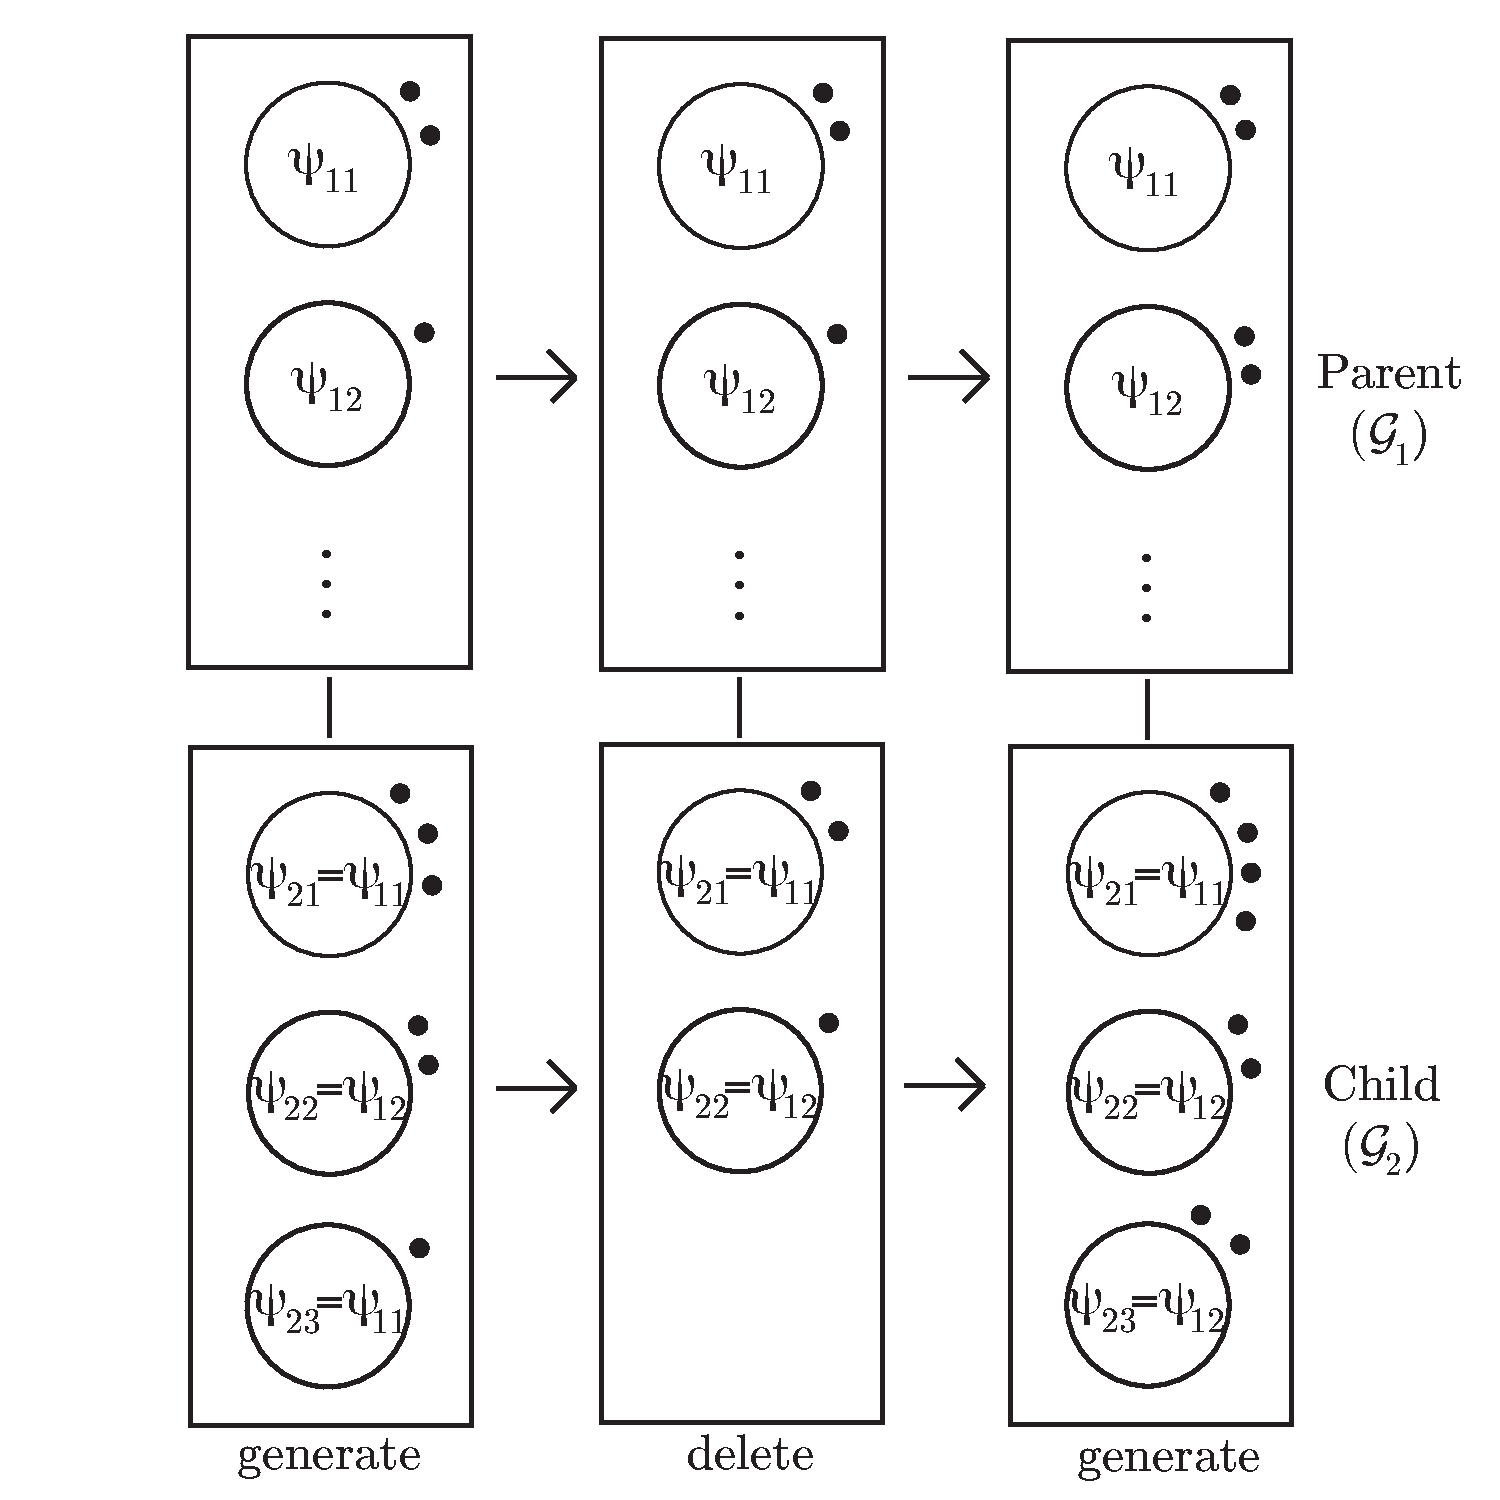
\includegraphics[height = 7cm]{../../papers/2010_icml/bounded_memory_compression/figure2.pdf}
		\end{center}
	\end{figure}
\end{frame}

\section{Experiments}


\begin{frame}[t]{Sequence Memoizer Computational Problems}
	Current state of the art results for inference in the sequence memoizer model are:
	\begin{itemize}
		\item Number of represented nodes grows as $\mathcal{O}(n)$ \cite{Wood2009}.  
		\begin{itemize}
			\item Since the model can be represented in space proportional to the number of represented nodes this corresponds to a linear complexity in space.
		\end{itemize}
		
		\item Prediction time grows as $\mathcal{O}(n)$ (empirically more like $\mathcal{O}(k)$ for non-adversarial data) \cite{Gasthaus2010}.
		\item Estimation time grows as $\mathcal{O}(n^2)$ (empirically more like $\mathcal{O}(n)$ for non-adversarial data) \cite{Gasthaus2010}.
	\end{itemize}
\end{frame}

\begin{frame}[t]{Example Prefix Tree: $patat$}
	\begin{center}
		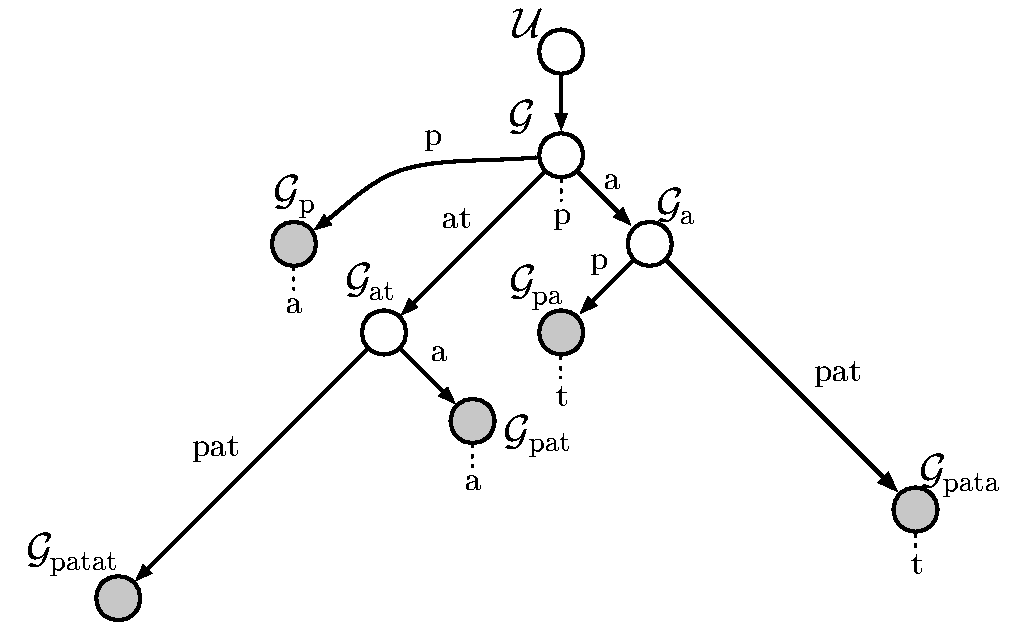
\includegraphics[width = 10cm]{../../papers/2010_icml/bounded_memory_compression/prefix_tree.pdf}
	\end{center}
\end{frame}

\begin{frame}[t]{Forget Some Data}
	Imagine that in the example prefix tree for $patat$, we ``forget" the observation $t$ in the context $pa$.  In this case, the node labeled $\G_{pa}$ no longer has any observations associated with it and will not need to be represented in the tree.
	
	\vspace{-.5cm}
	
	\begin{center}
		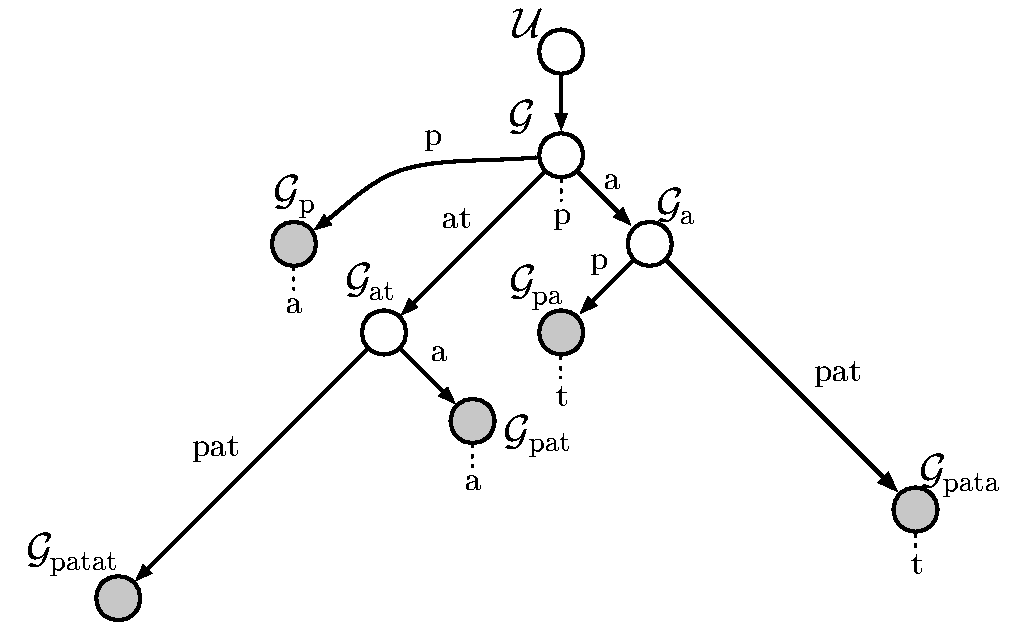
\includegraphics[height = 6cm]{../../papers/2010_icml/bounded_memory_compression/prefix_tree.pdf}
	\end{center}
\end{frame}

\begin{frame}[t]{Intuition}
	When could we ``forget" data in a Bayesian inference procedure?
	\begin{itemize}
		\item{If all the information from the observation $t$ in the context $pa$ regarding $\G_a$ is retained.}
		\item{$\G_{pa}$ before forgetting is assumed independent of $\G_{pa}$ after the forgetting.} 
	\end{itemize}
	
	\vspace{-.6cm}
	
	\begin{center}
		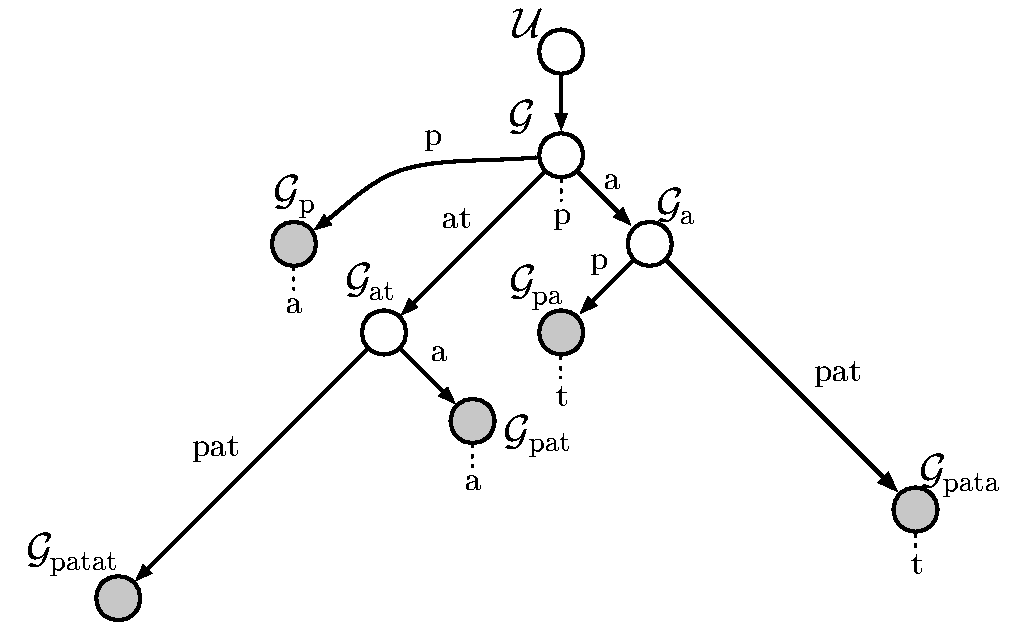
\includegraphics[height = 5.5cm]{../../papers/2010_icml/bounded_memory_compression/prefix_tree.pdf}
	\end{center}	
\end{frame}


\begin{frame}[t]{Task}
	\begin{block}{Prediction}
		Given a sequence of discrete observations $X_1, \ldots, X_n$, predict the next observation $X_{n+1}$.
	\end{block}
	
	\begin{block}{Requirements}
		\begin{itemize}
			\item{Linear time estimation in the length of the sequence}
			\item{Constant time prediction}
			\item{Constant space memory complexity}
		\end{itemize}
	\end{block}
\end{frame}


\begin{frame}[t]{Motivation: Streams}
	\begin{block}{Byte Stream}
		\[
		\begin{array}{l}
			01001001 , 01101110 , 00100000 , 01110100,\\
			01101000 , 01110010 , 01100101 , 01100101,\\
			00100000 , 01100100 , 01100001 , 01111001,\\
			01110010 , 01100001 , 01110011 , 01101000\ldots
		\end{array}
		\]
	\end{block}
	
	\begin{block}{Word Stream}
		the, rabbit, hole, went, straight, on, like, a, tunnel, for, some\\
		way, and, then, dipped, suddenly, down, so, suddenly, that\\
		alice, had, not, a, moment, to, think, about, stopping, herself\\
		before, she, found, herself, falling, down, a, very, deep, well
	\end{block}
\end{frame}



\begin{frame}[t]{Example Applications}
	\begin{itemize}
		\item{Natural Language}
		\begin{itemize}
			\item Words, i.e.~the united \_
			\item Characters, i.e.~un\_
			\item Parts of speech, i.e.~NNV\_
		\end{itemize}

		\vspace{.75cm}		
		
		\item{Compression}
		\begin{itemize}
			\item  Bits i.e.~0101000011110001\_
			\item  Bytes i.e.~6A7B4ED22100D\_
		\end{itemize}
		
		\item \ldots
	\end{itemize}
\end{frame}


\subsection{Constrained Memory}



\begin{frame}[t]{Constant Space Sequence Memoizer}
	\begin{figure}[t]
		\begin{center}
			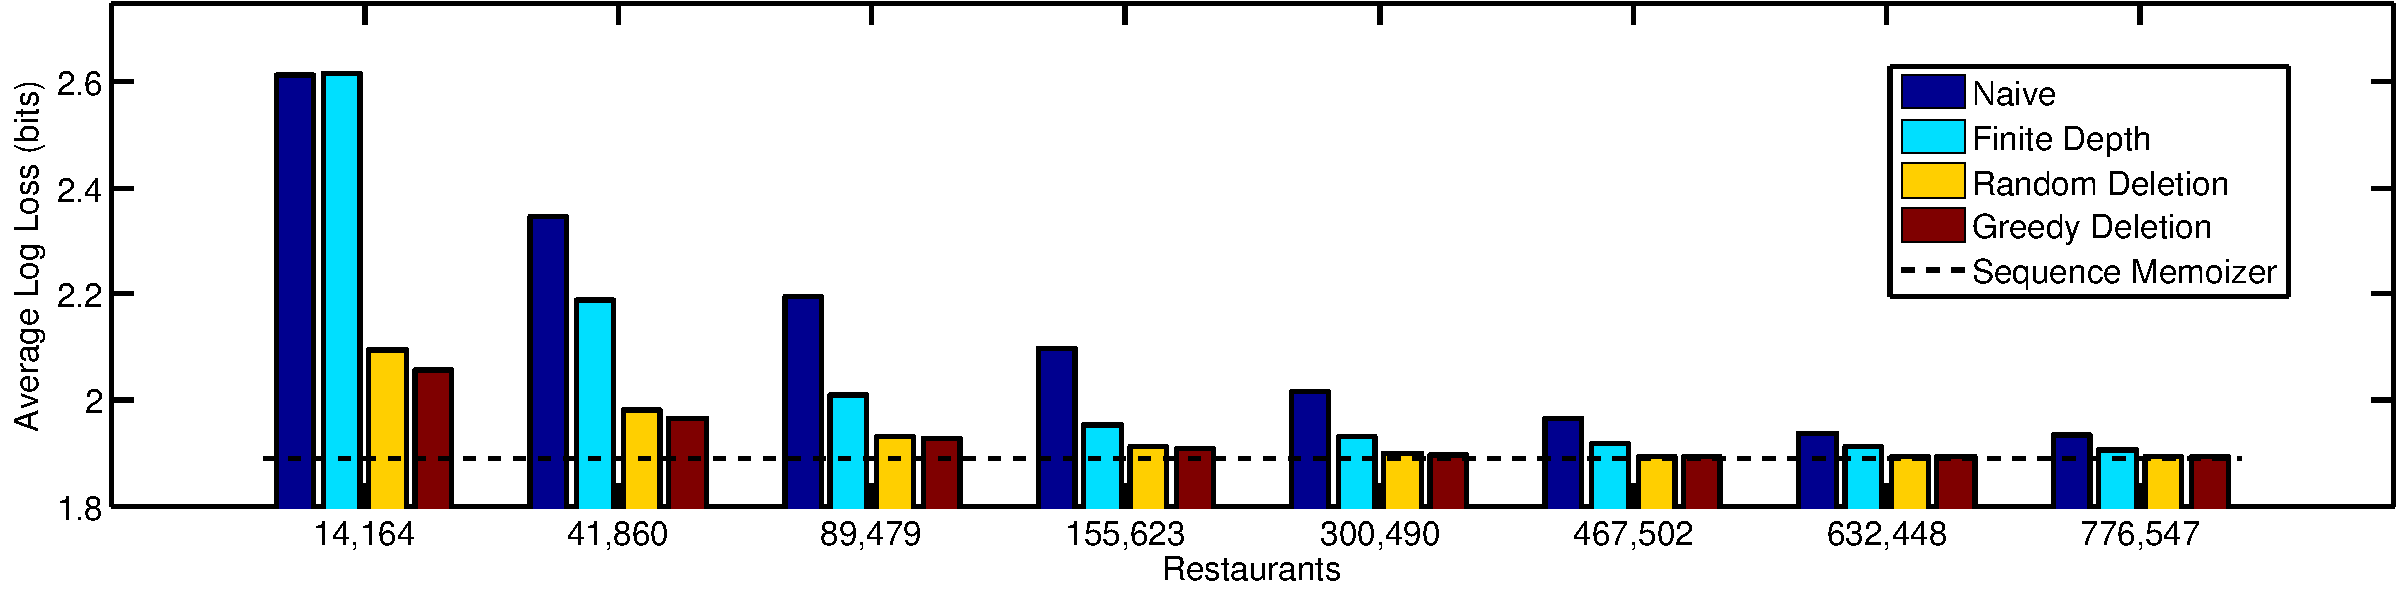
\includegraphics[width=10cm]{../../papers/2010_icml/bounded_memory_compression/results_calgary_corpus.pdf}
		\end{center}
	\end{figure}
	
	\begin{itemize}
		\item Calgary corpus
		\item Different forgetting schemes
		\item $256$ character alphabet
	\end{itemize}
	
	With random forgetting and 2 million instantiated nodes, we attain a compression rate of {\bf 1.49} bits per byte on the first 50 million bytes of the NYT Corpus.  The sequence memoizer can only process 1,488,233 bytes before needing to instantiate more than 2 million nodes, on the which the sequence memoizer attains a {\bf 1.72} bits per byte compression rate.
\end{frame}


\begin{frame}[t]{Constant Space Sequence Memoizer}
	\begin{figure}[t]
		\begin{center}
			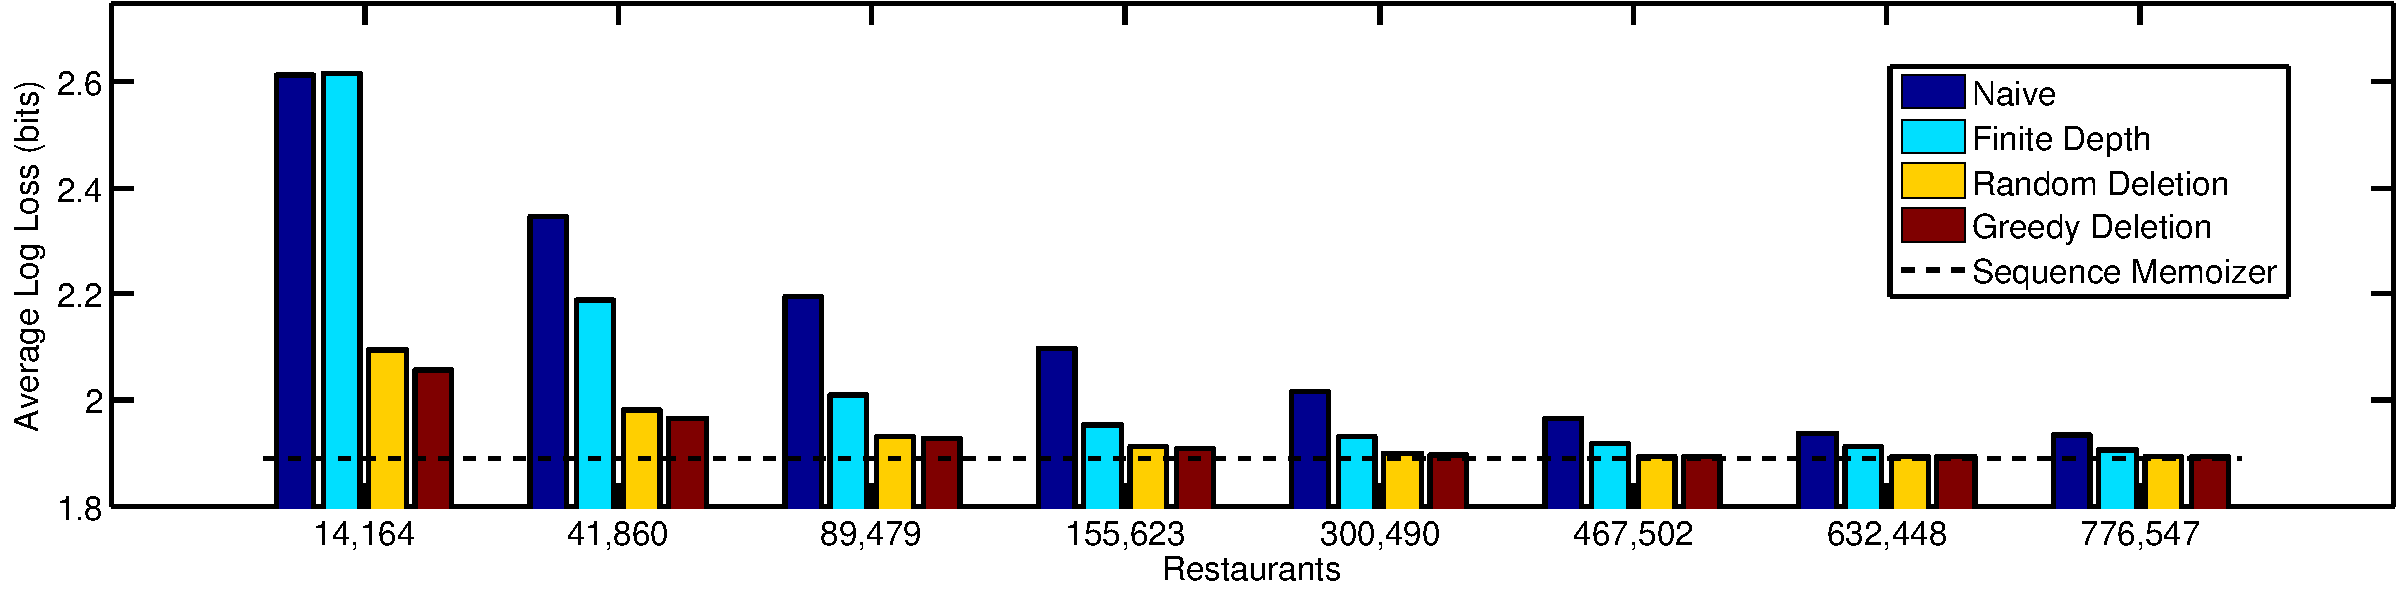
\includegraphics[width=10cm]{../../papers/2010_icml/bounded_memory_compression/results_calgary_corpus.pdf}
		\end{center}
	\end{figure}
	
	\begin{itemize}
		\item Calgary corpus
		\item Different forgetting schemes
		\item $256$ character alphabet
	\end{itemize}
\end{frame}
\section{Discussion}
\subsection{}
\begin{frame}[t]{Discussion}
	\begin{itemize}
		\item{The number of instantiated nodes can be limited using the deletion scheme developed for dependent HPYP�s. Memory savings can be achieved by deleting all the elements in a leaf node.}
		\item{Inference performed with forgetting estimates a dynamic stationary generative process.  Marginally the process is the same as the sequence memoizer model.}
		\item{Our deletion process requires us to assume the independence of a large number of distributions. While this may seem troubling, a key insight is that the entire set of distributions for which we must make the independence assumption are dependent on an existing node in the tree. Much of the information will be retained in the tree by the remaining node.}
	\end{itemize}
\end{frame}

\begin{frame}[t]{Thoughts}
	\begin{itemize}
		\item{Single particle particle filter}
		\item{Parametric model vs.~nonparametric model constrained to be constant space}
		\item{The resulting estimator may be inconsistent.  }
	\end{itemize}
\end{frame}

\begin{frame}[t,allowframebreaks]{Bibliograpy}
	\bibliography{../../papers/uber}
\end{frame}

\end{document}


